\begin{center}

\includegraphics[width=2.59in]{media/media/image1.png}

\vspace{0.35em}
\ddtitle{AURORA: Agentic UAV Refinement through\\
Optimization, Reflection, and Assurance}

\vspace{0.25em}
\textbf{Chi Zhang}
\end{center}

\begin{ddabstract}
UAV controller tuning in simulation is often framed as gain search, yet
a credible experiment must also bind every Candidate to an intended
scenario, finite budget, objective and constraint policy, trustworthy
execution, and holdout boundary. Foundation models can interpret intent
and coordinate methods, but a fluent response cannot prove that the
declared experiment actually ran. \textbf{AURORA---Agentic UAV Refinement
through Optimization, Reflection, and Assurance}---is the evidence-gated
Harness inside DroneDream 1.0. It compiles bounded context, filters tool
eligibility before routing, selects versioned optimizers or deterministic
fallbacks, executes from an immutable Trial, Candidate, and Job snapshot,
verifies claim receipt v3 and Outcome Contract 2.20, isolates fault and
holdout evidence, and freezes final selection only after deterministic
checks pass. Models may propose and route work; software contracts retain
authority over parameter domains, state transitions, evidence admission,
and completion. Evidence 2.7 additionally compiles one bounded
observational reflection from each verified decision cohort. It admits
accepted work, optimizer-learning Trials, domain failures, feasibility,
incumbent change, and observed improvement only when the execution
receipt and every modern Candidate receipt agree; any incomplete,
legacy, or drifted cohort makes the entire block unavailable, and no
association becomes causal tool credit. Frozen evidence records 1,139
backend tests in 759.17 seconds; its receipt marks the full suite as a
pre-commit run and binds a 59-check focused bridge to the software
subject commit. The separate Windows Rust gate was not run.
Current software evidence records 16/16 deterministic policy-holdout
checks, 25/25 source-contract probes versus 6/25 with weakened guards,
and 10/10 matched fallback comparisons across a 15-Job, 579-Trial
synthetic campaign. A separate frozen four-arm component ablation spans
20 Jobs and 554 Trials with complete evidence and zero network access;
its receipt-only-memory isolation is explicitly inconclusive in 5/5
seed blocks. The archived 24/24 provider-routing result remains valid
only for Evidence 2.4 and Prompt 1.1. These results validate exercised
routing, provenance, reflection, and recovery contracts; they do not
prove general optimizer superiority, physical simulator quality,
real-aircraft safety, or simulation-to-reality transfer. A fresh online
provider freeze for Evidence 2.7 and Prompt 1.5 and a matched multi-seed
PX4/Gazebo outcome campaign remain explicit qualification gates before
either optimization quality or simulator fidelity can be claimed in
customer deployment.

\vspace{0.35em}
\href{https://github.com/ChiZhang-805/DroneDream}{
\raisebox{-0.12em}{
\includegraphics[height=0.9em]{media/github-mark.png}}
\enspace github.com/ChiZhang-805/DroneDream}
\end{ddabstract}

\section{\texorpdfstring{\textbf{1.
Introduction}}{1. Introduction}}\label{introduction}

UAV controller tuning is not a single-number search. PX4 layers rate,
attitude, velocity, and position controllers, and useful gains shift with
propulsion, mass, assembly, and scenario conditions. Its official workflow
therefore remains iterative: apply parameters, excite the system, inspect
the response, and revise. Software-in-the-loop changes the risk and cost
of that loop, not its combinatorics. A credible campaign must choose a
method and finite budget, preserve scenario identity, evaluate objectives
and constraints, distinguish parameter failure from infrastructure fault,
and reserve unseen scenarios for final selection. Derivative-free and
Bayesian methods systematize search, from reusable services to
trust-region and sparse high-dimensional variants
{[}\protect\hyperlink{ref_2}{\emph{2}}, \protect\hyperlink{ref_3}{\emph{3}}, \protect\hyperlink{ref_4}{\emph{4}}, \protect\hyperlink{ref_5}{\emph{5}}, \protect\hyperlink{ref_6}{\emph{6}}, \protect\hyperlink{ref_7}{\emph{7}}, \protect\hyperlink{ref_8}{\emph{8}}{]},
but still assume a correctly formed experiment. They neither translate
engineering intent into an auditable program nor prove that its declared
conditions were executed as declared in its persisted manifest.

Foundation models provide a useful interface layer, but not experimental
authority. Tool-using agent systems show that model reasoning becomes
more effective when coupled to explicit tools, machine-readable state,
feedback, reflective memory, and bounded execution interfaces
{[}\protect\hyperlink{ref_16}{\emph{16}},
\protect\hyperlink{ref_17}{\emph{17}},
\protect\hyperlink{ref_28}{\emph{28}},
\protect\hyperlink{ref_29}{\emph{29}},
\protect\hyperlink{ref_30}{\emph{30}}{]}. In control optimization,
however, a plausible explanation cannot prove that a scenario was
applied, a metric came from the intended trial, or a final candidate
remained isolated from holdout leakage. Those facts must come from
deterministic software and retained evidence. AURORA (Agentic UAV
Refinement through Optimization, Reflection, and Assurance), the
evidence-gated Harness inside DroneDream 1.0, therefore uses model
intelligence to interpret the task and rank specialized methods, while
deterministic compilers, versioned contracts, simulator receipts, outcome
taxonomy, and a final freeze gate authorize every consequential
transition. The model may propose the next action; it cannot declare
that action executed or promote an unverified observation. AURORA
therefore compiles conversation into a bounded optimization program
whose claims are earned by retained evidence.
\looseness=-1

This report makes three contributions. First, it specifies the system
boundary that separates model reasoning, tool eligibility, simulation
execution, and evidence authority. Second, it reports reproducible
routing, guard, fallback, and synthetic integration evidence without
relabeling software contracts as physical performance. Third, it defines
the experiments still required before broader simulator-quality claims
are justified. The presentation follows the causal narrative common to
modern technical reports in agentic and embodied AI
{[}\protect\hyperlink{ref_15}{\emph{15}},
\protect\hyperlink{ref_18}{\emph{18}},
\protect\hyperlink{ref_19}{\emph{19}}{]}, while keeping DroneDream's
claims tied to its own frozen artifacts and independently auditable
release boundary for independent regeneration or reuse.

\subsection{\texorpdfstring{\textbf{1.1 Product
scope}}{1.1 Product scope}}\label{product-scope}

The product boundary is simulation-first. The desktop application guides
scenario design, experiment planning, execution, evidence review,
recovery, and reporting. The public website explains and distributes the
product, hosts documentation and community features, and exposes
subscription entry points. Supabase supplies identity, community data,
quota accounting, and the managed-model gateway; DroneDream 1.0 keeps
PX4/Gazebo simulation local to the owned Runtime. The boundary is
equally explicit about what is not claimed: this report does not certify
real-aircraft safety, guarantee simulation-to-reality transfer, or
authorize unbounded autonomous flight actions. A model may propose or
route work, but it may not convert an unverified result into
a completed tuning outcome. AURORA must earn that transition with evidence.

\section{\texorpdfstring{\textbf{2. Related work and design
rationale}}{2. Related work and design rationale}}\label{related-work-and-design-rationale}

\textbf{Black-box optimization supplies the search machinery, but not
the experimental constitution.} CMA-ES provides a robust derivative-free
evolutionary strategy, while Vizier and BoTorch formalize reusable
optimization services and modern Bayesian-optimization primitives. TuRBO
addresses local search in high dimensions, and SAASBO models sparse
axis-aligned structure {[}\protect\hyperlink{ref_4}{\emph{4}},
\protect\hyperlink{ref_5}{\emph{5}},
\protect\hyperlink{ref_6}{\emph{6}},
\protect\hyperlink{ref_7}{\emph{7}},
\protect\hyperlink{ref_8}{\emph{8}}{]}. Efficient Global Optimization
established the surrogate-and-acquisition loop for expensive black-box
functions, practical Bayesian optimization showed how to carry that loop
into noisy model selection, and the field review makes the remaining
choices around priors, acquisition, constraints, and parallelism
explicit {[}\protect\hyperlink{ref_31}{\emph{31}},
\protect\hyperlink{ref_32}{\emph{32}},
\protect\hyperlink{ref_33}{\emph{33}}{]}. These methods motivate
DroneDream's portfolio, yet each remains conditional on a correctly
specified objective, feasible domain, trial budget, and trustworthy
observation stream. DroneDream's distinct engineering problem begins one
level above the optimizer: it must decide which method is eligible,
prove which scenario was actually applied, and prevent infrastructure
faults or holdout outcomes from entering the learning history or
contaminating any later comparison.

\textbf{Robotic foundation models demonstrate broad semantic and action
priors, but they solve a different authority problem.} RT-1 and RT-2
established large-scale vision-language-action learning; Open
X-Embodiment and OpenVLA expanded cross-embodiment data and open model
access; \(\pi_0\) and \(\pi_{0.5}\) explored flow-based action generation and
heterogeneous co-training; JoyAI-RA continued this line with a
multi-source autonomy foundation model
{[}\protect\hyperlink{ref_9}{\emph{9}},
\protect\hyperlink{ref_10}{\emph{10}},
\protect\hyperlink{ref_11}{\emph{11}},
\protect\hyperlink{ref_12}{\emph{12}},
\protect\hyperlink{ref_13}{\emph{13}},
\protect\hyperlink{ref_14}{\emph{14}},
\protect\hyperlink{ref_15}{\emph{15}},
\protect\hyperlink{ref_20}{\emph{20}},
\protect\hyperlink{ref_21}{\emph{21}},
\protect\hyperlink{ref_27}{\emph{27}}{]}. DroneDream does not claim an
end-to-end flight policy or place a language model in the control loop.
It uses model reasoning only to interpret intent and rank eligible
tools; deterministic software retains authority over experiment
construction, simulator execution, evidence admission, final selection,
release, and rollback.

\textbf{Data scale and benchmark breadth have advanced faster than
evidence semantics.} Open X-Embodiment, BridgeData V2, DROID, and AgiBot
World expand the diversity of robot experience; RoboCasa and RoboTwin
2.0 scale simulation tasks and controlled perturbations
{[}\protect\hyperlink{ref_11}{\emph{11}},
\protect\hyperlink{ref_22}{\emph{22}},
\protect\hyperlink{ref_23}{\emph{23}},
\protect\hyperlink{ref_24}{\emph{24}},
\protect\hyperlink{ref_25}{\emph{25}},
\protect\hyperlink{ref_26}{\emph{26}}{]}. These resources strengthen
policy training and comparative evaluation, but their success metrics do
not answer whether a local UAV tuning run applied the intended scenario,
whether a failed trial was physical or infrastructural, or whether
holdout evidence leaked back into search. DroneDream therefore treats
dataset coverage, optimizer quality, and evidence validity as independent
axes: benchmark breadth or policy scores cannot substitute for evidence
about the exact experiment that generated a reported result.
\looseness=-1

\textbf{Tool-using agents clarify why that separation matters.}
SWE-agent shows the value of an explicit agent-computer interface, and
AlphaEvolve couples model proposals to evaluators and an evolutionary
loop {[}\protect\hyperlink{ref_16}{\emph{16}},
\protect\hyperlink{ref_17}{\emph{17}},
\protect\hyperlink{ref_28}{\emph{28}},
\protect\hyperlink{ref_29}{\emph{29}},
\protect\hyperlink{ref_30}{\emph{30}}{]}. ReAct interleaves reasoning
with environmental actions; Toolformer studies learned tool invocation;
Reflexion uses feedback as episodic memory. Together they locate
capability in interfaces, evaluators, and feedback loops. DroneDream
adopts that interface principle but never treats free-form reflection as
experimental evidence. Only structured, provenance-bound,
policy-eligible outcomes may update decision memory; failure taxonomy,
holdout isolation, and the final freeze gate prevent generated narratives
from replacing the versioned simulator receipts and outcome records that support a claim.
\looseness=-1

\section{\texorpdfstring{\textbf{3. System and
method}}{3. System and method}}\label{system-and-method}

\textbf{The architecture assigns a single authority to every
transition.} The desktop owns user intent and interaction; the FastAPI
backend and worker validate job transitions and persist bounded state;
the AURORA compiles context, filters tool eligibility, and admits only
trusted outcomes; the owned Runtime supplies pinned PX4/Gazebo
dependencies; and cloud services provide identity, community data, quota
accounting, and a managed-model gateway without exposing the platform
key to clients. Separating these roles prevents a router choice from
becoming an executable experiment until deterministic compilers,
validators, and Runtime probes agree on the same versioned contract
before launch or retry.

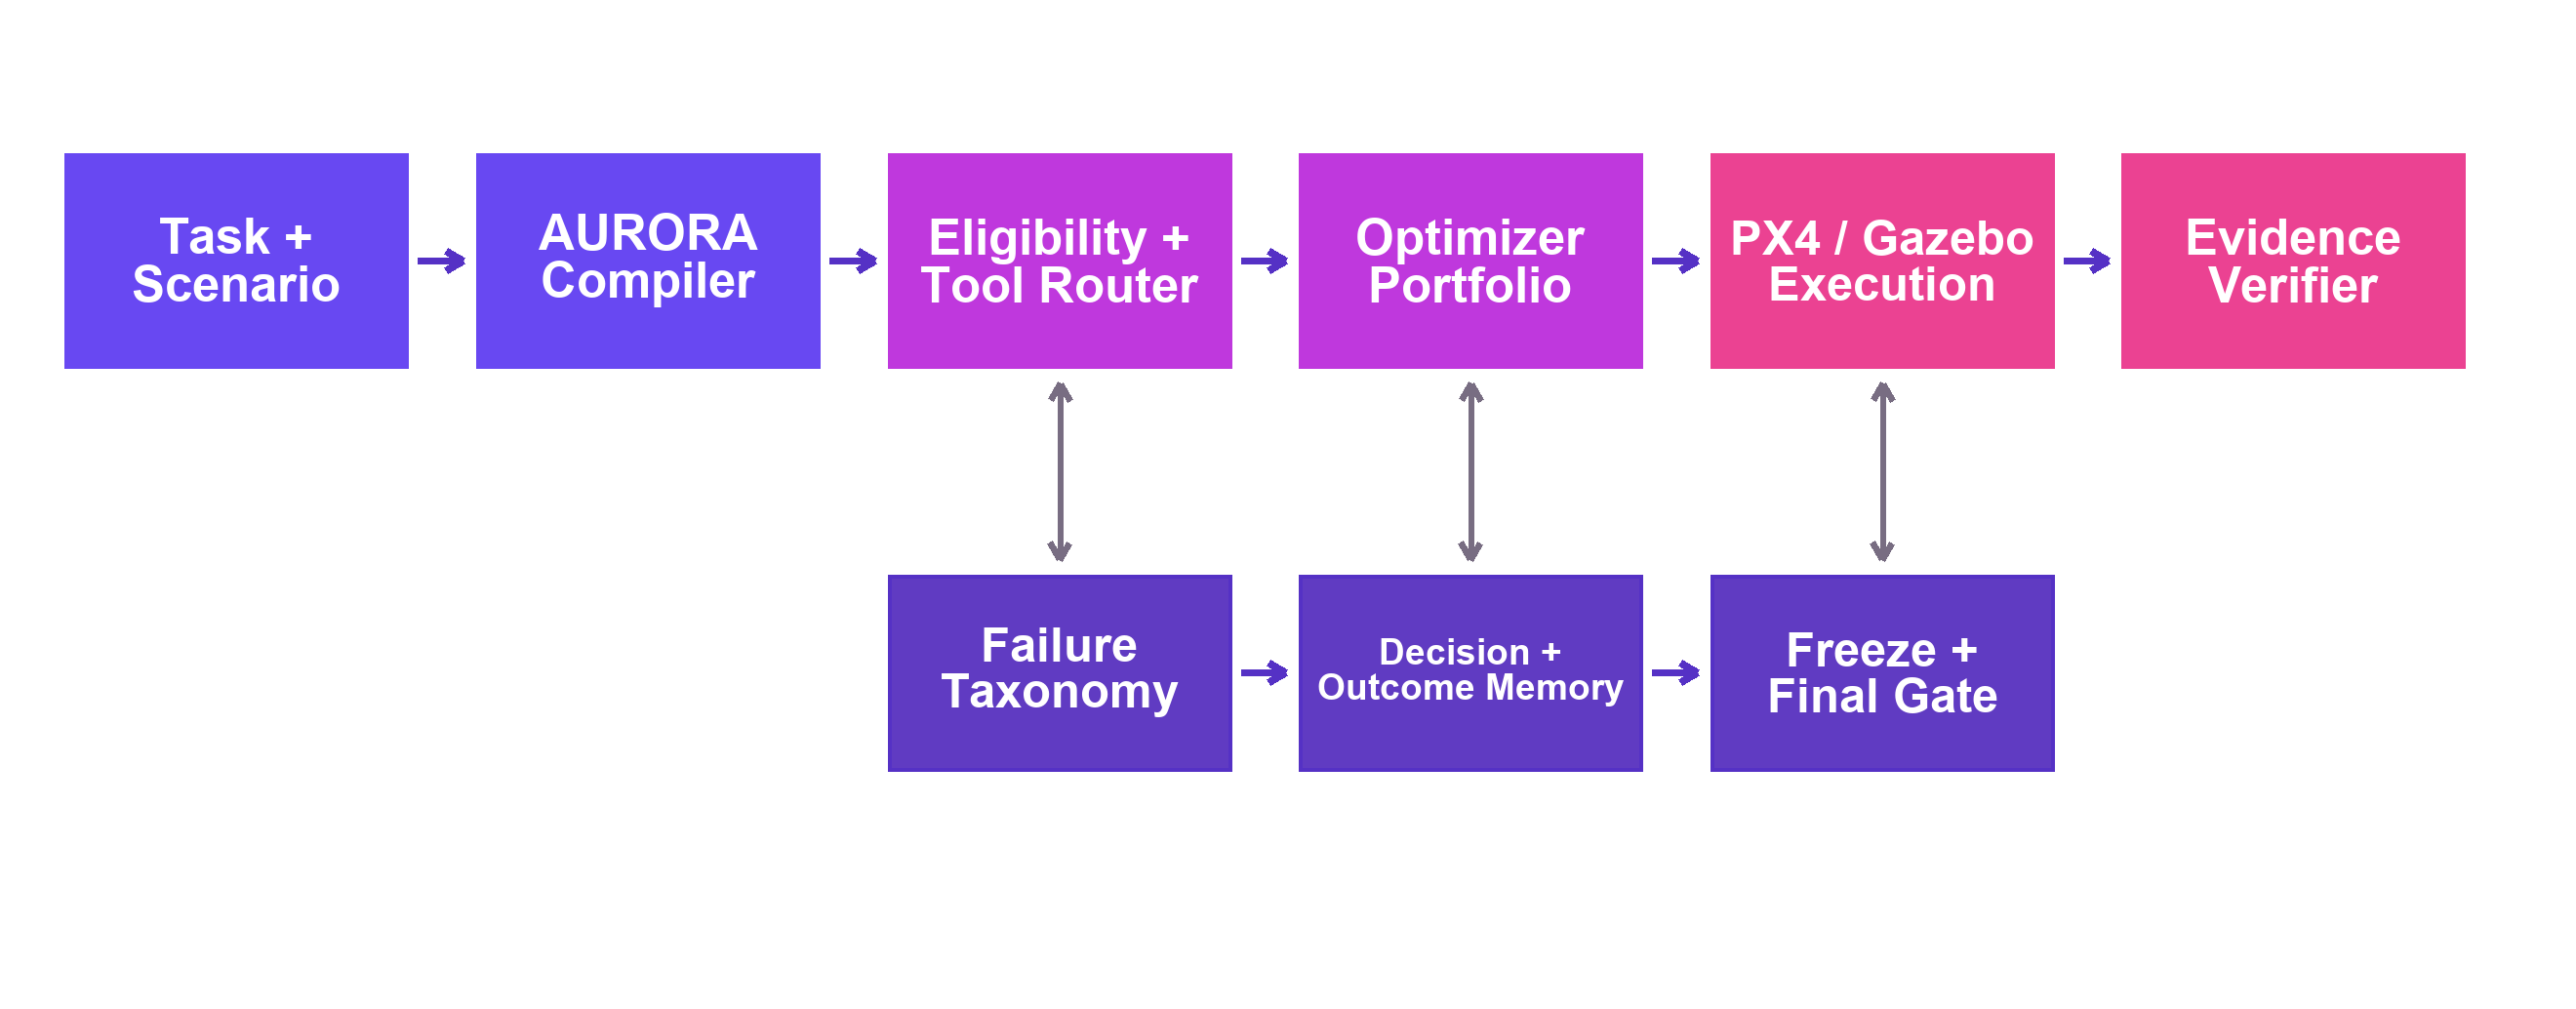
\includegraphics[width=6.50000in,height=2.54583in]{media/media/image3.png}

\emph{Figure 1. AURORA's evidence-gated optimization loop inside
DroneDream 1.0. Provenance-complete, policy-eligible outcomes alone may
influence routing memory or pass the final selection gate.}

\begin{itemize}
\item
  Desktop boundary --- readiness, user input, progress, settings, and
  safe exit;
  entry remains hidden while any required launch check is pending or
  failed across every required readiness stage.
\item
  Backend boundary --- drafts, jobs, orchestration, APIs,
  and artifacts; only validated state transitions and stable failure
  codes are accepted before persistence, dispatch, or artifact
  publication.
\item
  AURORA authority --- context, eligibility, routing, reflection, and
  evidence memory;
  only provenance-complete evidence may influence a decision during routing and final selection.
\item
  Runtime boundary --- PX4/Gazebo and pinned dependencies; declared
  versions are insufficient without effect and source evidence from the
  launched process, accepted customer Runtime, and published release
  ledger.
\item
  Cloud boundary --- authentication, community data, quota ledger, and
  model
  gateway; provider secrets remain server-side and never enter desktop
  logs or artifacts under any subscription tier.
\end{itemize}

\subsection{\texorpdfstring{\textbf{3.1 AURORA: the evidence-gated
Harness}}{3.1 AURORA: the evidence-gated Harness}}\label{aurora-the-evidence-gated-harness}

\textbf{AURORA is a constrained decision system around simulation.}
Context binds parameters, scenarios, history, budgets, and failures.
Capability eligibility removes incompatible tools, while a phase gate
exposes only methods suited to exploration, recovery, refinement,
diversification, or verification. The router ranks that executable
surface and the optimizer proposes Candidates. Verification forces every
reduced-fidelity strategy to fidelity 1.0 before acceptance.
Provenance-bound memory admits trusted outcomes, while the final gate
freezes holdout results and rejects incomplete artifacts. Each stage
narrows authority, so fluent output cannot bypass an executable contract
or test.

\textbf{Claim-time inputs are immutable before launch.} Schema
\textbf{dronedream.trial-execution-attempt-claim/v3} and digest
\textbf{execution\_input\_sha256} bind Trial, Candidate, and Job inputs
in one snapshot. Outcome Contract 2.20 authorizes the scenario matrix
and constructs \textbf{TrialContext} without rereading mutable rows.
Checks classify changed inputs as \textbf{INPUT\_EVIDENCE\_DRIFT},
coordinated rewrites as \textbf{OUTCOME\_CONTRACT\_DRIFT}, and
unauthorized fields as \textbf{SCENARIO\_CONTRACT\_DRIFT}. Completion
locks Job
before Trial; historical receipts remain verifiable, new claims use v3,
and the original projection stays available for audit replay under the
same claim boundary.

\textbf{Physical claims are concurrency-safe and fairly scheduled.}
Execution Claim Gate 1.1 combines PostgreSQL FOR UPDATE SKIP LOCKED, a
conditional lease update, bounded retries, and an attempt-count fence.
Eight concurrent workers yield one physical execution and one accepted
outcome for a logical Trial, with no duplicate evidence in an
eight-Trial pool. Scheduling Gate 1.0 chooses the least-served eligible
Job and preserves FIFO within it. A two-Job regression makes six
sequential claims alternate, preventing
desktop-lane monopoly; hosted priority and resource-cost scheduling
remain outside the current local scheduling contract, audit replay, and
evidence envelope for hosted work.

\textbf{Model feedback is case-separated.}
Prompt Schema 2.3 assigns provider-safe
\mbox{training\_case\_N} aliases in
frozen order, keeping same-type cases with different weights or numeric
configurations distinct. Each admitted case carries its weight, seed
count, metrics, and closed failure counts; raw IDs, unsupported text,
and holdout evidence stay outside the prompt. This removes
feedback-grouping ambiguity without expanding model authority or
claiming simulator
fidelity, and preserves canonical order when matched Trials arrive in
reverse. The separation is preserved in every provider request and
retained routing receipt for later independent inspection and audit
replay across reruns and reviews over time.

\textbf{Reproducibility extends below the random seed.} A non-unique
eigenvector factor can rotate an identical seeded normal sample when
another BLAS kernel resolves repeated covariance eigenvalues
differently. DroneDream instead uses the unique symmetric
positive-definite covariance square root and canonical unit-vector
spelling before discrete projection. The frozen optimizer transcript
hashes executed candidates, losses, feasibility,
route, fidelity, and cohort position, while non-causal GP/CMA diagnostic
matrices remain outside that decision hash
{[}\protect\hyperlink{ref_1}{\emph{1}}{]}. This boundary lets supported
machines replay identical candidate sequences across machines before any
provider decision receives credit.

\textbf{Feedback is verified again at the model boundary.} Optimizers,
the closed-tool router, and direct proposer share one training-feedback
compiler. It reconstructs canonical Trial rows and checks the
content-addressed outcome against Candidate identity, generation,
parameters, and Trial evidence before exposing a score. Sibling fields
cannot override those values. Divergence is quarantined rather than
turned into a bad-parameter penalty; migration-era rows remain
explicitly
unsealed and ineligible for learning, routing memory, or final selection
{[}\protect\hyperlink{ref_1}{\emph{1}}{]}. The rule preserves
auditability across both current and migration-era experiment histories
and their later replay without retroactive reinterpretation.

Reflection is compiled from verified outcomes rather than free-form
model self-report. Evidence 2.7 joins one accepted execution receipt to
the exact optimizer Candidate cohort for that generation, then requires
every Candidate to carry a current v2 evidence receipt and verified
training feedback. Prompt 1.5 and Decision Trace 1.3 also bind the exact
phase-qualified tool surface. The bounded \textbf{observed\_outcome} block records
cohort size, accepted attempts, optimizer-learning Trials, domain
failures, feasible Candidates, completion rate, the incumbent before and
after the cohort, and observed absolute and relative improvement. A
count mismatch, incomplete result, legacy record, or evidence drift
makes the whole block \textbf{unavailable}; a zero-dispatch decision is
explicitly not applicable. Holdout measurements, private identifiers,
seeds, hashes, and failure prose remain outside provider-visible memory.
The prompt treats these values only as bounded temporal associations:
reflection may guide the next decision, but it cannot assign causal
reward or portfolio-child credit unless a separately controlled intervention supports that claim.
\looseness=-1

\begin{itemize}
\item
  COMPLETED with a usable metric is admitted as successful optimizer
  evidence.
\item
  FAILED with a trusted domain failure code is admitted as a
  non-success because it may identify an infeasible or unsafe simulated
  parameter region without being mislabeled as infrastructure failure.
\item
  Infrastructure faults, cancellation, malformed evidence, and
  conflicting terminal states are quarantined and cannot update search
  or routing memory under any later decision path or replay.
\item
  Holdout-only outcomes are
  reserved for final evaluation and are never returned to the training history.
\end{itemize}

Infrastructure failures, cancellation, malformed or internally
conflicting evidence, and holdout-only outcomes are isolated from
optimizer learning and routing memory. Admission requires a terminal
state, an allowed domain failure code where applicable, a
content-addressed Candidate-to-Trial match, and complete provenance for
the executed scenario. Rejected rows retain a stable quarantine reason
for diagnosis but cannot update scores, route preferences, recovery
memory, or the next candidate proposal. This evidence boundary prevents
a simulator crash, stale callback, or evaluation-only result from being
learned as if it described the quality of a parameter set. The retained
experiment ledger makes every quarantine decision independently
inspectable without allowing the rejected observation to affect later search.
\looseness=-1

\section{\texorpdfstring{\textbf{4. Experiments and
evidence}}{4. Experiments and evidence}}\label{experiments-and-evidence}

This section keeps unlike evidence units separate. Development and
policy-holdout corpora test tool eligibility; source ablations test
named guards; the fallback campaign tests recovery equivalence under a
fixed mock budget; and synthetic integration tests orchestration on a
declared non-physical objective. Every result is recomputed from
persisted records and paired with a claim boundary. PX4/Gazebo
assertions remain isolated until the signed customer Runtime passes a
provenance-bound acceptance campaign, preventing software
checks and proxy outcomes from being pooled into one headline score or
silently promoted beyond their declared evidence class in any
publication-facing claim.

\subsection{\texorpdfstring{\textbf{4.1 Development routing
evidence}}{4.1 Development routing evidence}}\label{development-routing-evidence}

The archived 24-case artifact spans eight routing categories and binds
its corpus, Evidence 2.4 inputs, Prompt 1.1, model snapshot, parser, and
scoring rule. Every case declares an acceptable selection set before
execution, and the report recomputes 24/24 from persisted per-case
records. The artifact therefore remains valid historical development
evidence for that exact contract, but it is not current qualification
for Evidence 2.7 and Prompt 1.5, which add verified observed-outcome
reflection. This result establishes bounded internal consistency; it
does not establish lower simulator loss, superiority to a learned
baseline, or generalization to
unseen tasks, vehicles, scenarios, provider outputs, or the revised prompt contract.

\begin{longtable}[]{@{}L{0.32\linewidth}C{0.19\linewidth}L{0.36\linewidth}@{}}
\caption{Archived routing accuracy and claim boundary}\tabularnewline
\toprule
\textbf{Comparator} & \textbf{Acceptable selections} & \textbf{Evidence
treatment}\tabularnewline
\midrule
\endhead
Archived AURORA router & 24/24 & Evidence 2.4 / Prompt 1.1
only\tabularnewline
Best constant policy & 14/24 & Deterministic corpus
baseline\tabularnewline
Uniform random expectation & 5.625/24 & Analytical
expectation\tabularnewline
\bottomrule
\end{longtable}

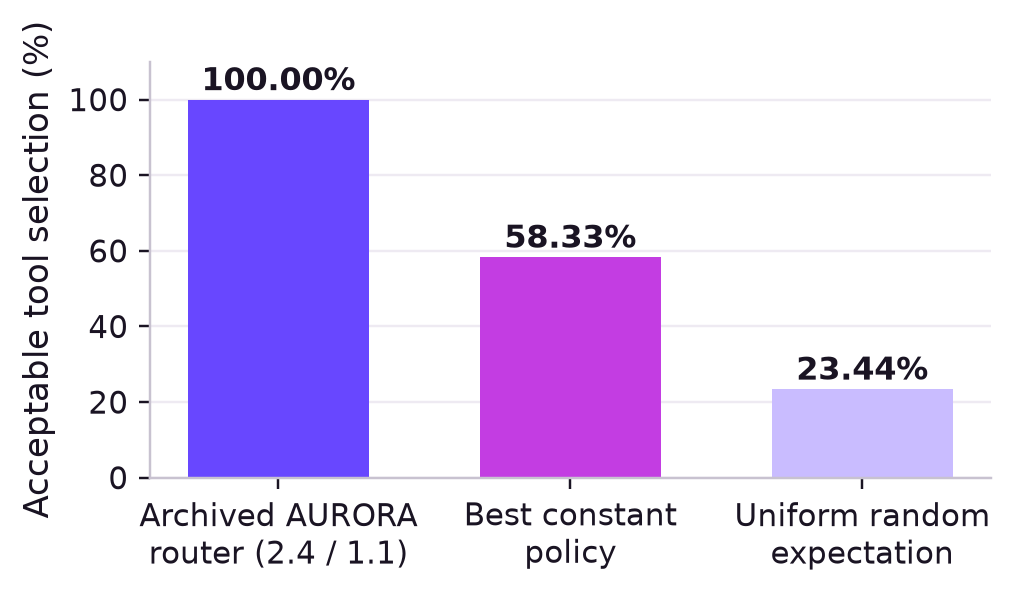
\includegraphics[width=4.35000in,height=2.56186in]{media/media/image4.png}

\emph{Figure 2. Archived acceptable tool selection under Evidence 2.4
and Prompt 1.1. The 24-case development result measures contract-specific
routing consistency, not current qualification or simulator outcomes.}

\subsection{\texorpdfstring{\textbf{4.2 Deterministic routing-policy
holdout}}{4.2 Deterministic routing-policy holdout}}\label{deterministic-routing-policy-holdout}

A separate 16-case corpus freezes exact eligible-tool sets at capability
boundaries and binds the corpus, case IDs, compiled policy inputs, and
development-corpus hash. It passes 16/16 exact comparisons. The runner
performs zero model calls, simulator runs, or feedback writebacks, and a
central flow guard rejects use of these results as prompt examples,
training data, development evidence, or runtime feedback. Cases exercise
dimension, constraint, multi-objective, fidelity, feasible-history, and
restart boundaries so the exact-set assertion detects both an
incorrectly admitted tool and an incorrectly excluded one. Because
labels become visible when the repository is published, this artifact
verifies deterministic
policy behavior but is not described as a permanently blind benchmark.
\looseness=-1

\begin{longtable}[]{@{}L{0.20\linewidth}C{0.25\linewidth}L{0.42\linewidth}@{}}
\caption{Deterministic routing-policy holdout}\tabularnewline
\toprule
\textbf{Measure} & \textbf{Result} & \textbf{Claim
boundary}\tabularnewline
\midrule
\endfirsthead
\toprule
\textbf{Measure} & \textbf{Result} & \textbf{Claim
boundary}\tabularnewline
\midrule
\endhead
\vtop{\hbox{\strut Eligible-tool}\hbox{\strut sets}} &
\vtop{\hbox{\strut 16/16 exact}\hbox{\strut matches}} &
\vtop{\hbox{\strut Current production}\hbox{\strut eligibility
only}}\tabularnewline
\vtop{\hbox{\strut External}\hbox{\strut activity}} &
\vtop{\hbox{\strut 0 calls; 0}\hbox{\strut simulator runs}} &
\vtop{\hbox{\strut No model or
outcome}\hbox{\strut evidence}}\tabularnewline
\vtop{\hbox{\strut Adaptive}\hbox{\strut writeback}} &
\vtop{\hbox{\strut 0; flow guard}\hbox{\strut rejects}} &
\vtop{\hbox{\strut Evaluation
artifact}\hbox{\strut only}}\tabularnewline
\vtop{\hbox{\strut Label}\hbox{\strut visibility}} &
\vtop{\hbox{\strut Published with}\hbox{\strut repository}} &
\vtop{\hbox{\strut Not permanently}\hbox{\strut blind}}\tabularnewline
\bottomrule
\end{longtable}

\subsection{\texorpdfstring{\textbf{4.3 AURORA source-contract
ablations}}{4.3 AURORA source-contract ablations}}\label{aurora-source-contract-ablations}

The ablation suite asks a narrow question: whether each named source
guard changes an otherwise identical deterministic decision at the
boundary it is designed to protect. For every guard, the production
contract and one intentionally weakened comparator receive the same
fixed probes, expected result, and scoring rule. Production satisfies
25/25 probes, whereas the matched weakened variants satisfy 6/25 after
their designated protection is removed. This construction demonstrates
enforceable behavior for fallback, provider trust, outcome isolation,
and tool eligibility; it is not a statistical effect estimate and does
not measure optimizer quality, simulated control performance, flight
safety, or readiness.

\begin{longtable}[]{@{}L{0.18\linewidth}L{0.36\linewidth}C{0.10\linewidth}C{0.11\linewidth}C{0.11\linewidth}@{}}
\caption{AURORA source-contract ablations}\tabularnewline
\toprule
\textbf{Guard} & \textbf{Protected boundary} & \textbf{Cases} &
\textbf{Production} & \textbf{Weakened}\tabularnewline
\midrule
\endfirsthead
\toprule
\textbf{Guard} & \textbf{Protected boundary} & \textbf{Cases} &
\textbf{Production} & \textbf{Weakened}\tabularnewline
\midrule
\endhead
\vtop{\hbox{\strut deterministic}\hbox{\strut fallback}} &
\vtop{\hbox{\strut Provider-independent}\hbox{\strut recovery path}} & 4
& 4/4 & 1/4\tabularnewline
\vtop{\hbox{\strut provider trust}\hbox{\strut filter}} &
\vtop{\hbox{\strut Trusted provider evidence}\hbox{\strut enters
decisions}} & 5 & 5/5 & 2/5\tabularnewline
\vtop{\hbox{\strut scenario/outcome}\hbox{\strut isolation}} &
\vtop{\hbox{\strut Holdout and fault evidence}\hbox{\strut stay outside
learning}} & 6 & 6/6 & 2/6\tabularnewline
\vtop{\hbox{\strut scenario profile}\hbox{\strut context}} &
\vtop{\hbox{\strut Profile evidence enters}\hbox{\strut every decision}} & 5
& 5/5 & 0/5\tabularnewline
\vtop{\hbox{\strut tool eligibility}\hbox{\strut gate}} &
\vtop{\hbox{\strut Incompatible tools}\hbox{\strut remain blocked}} & 5
& 5/5 & 1/5\tabularnewline
\bottomrule
\end{longtable}

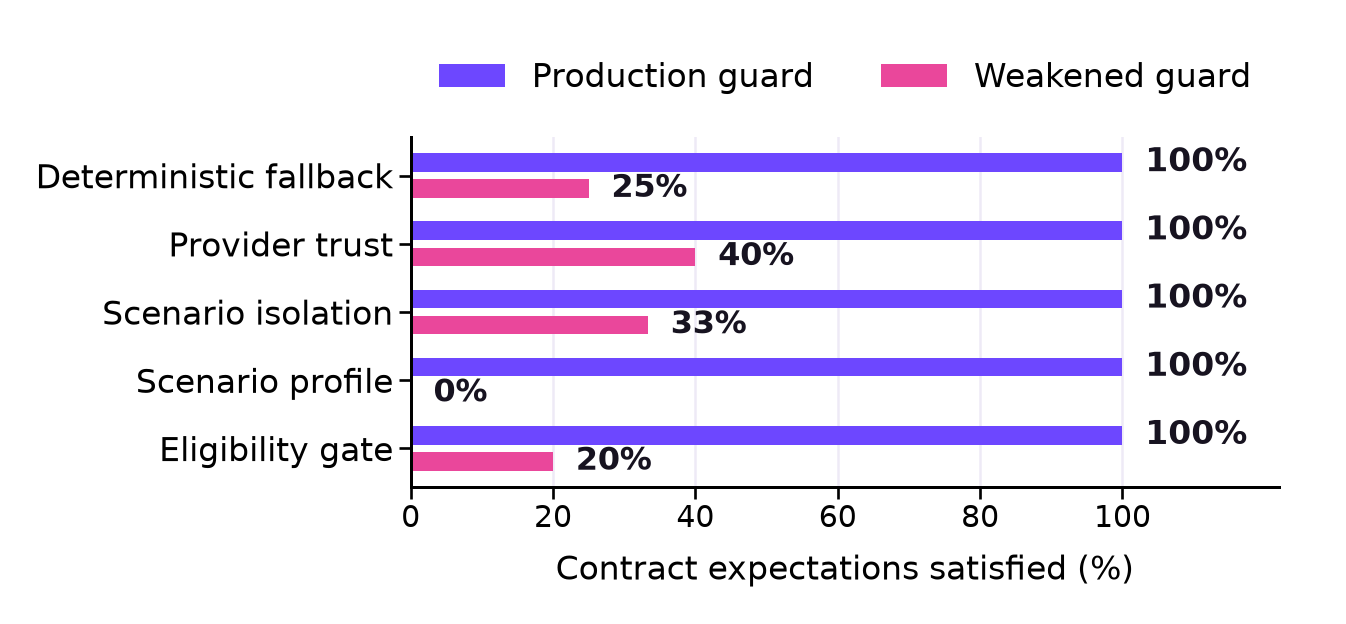
\includegraphics[width=5.10000in,height=2.36000in]{media/media/image5.png}

\emph{Figure 3. Constructed deterministic software-contract probes for
each AURORA guard. The weakened comparison measures fail-closed boundary
enforcement, not simulator performance or causal effect.}

\subsection{\texorpdfstring{\textbf{4.4 Fail-closed outcome
equivalence}}{4.4 Fail-closed outcome equivalence}}\label{fail-closed-outcome-equivalence}

Five fixed seed blocks compare three matched-budget arms: direct
portfolio, provider-error fallback, and invalid-response fallback. The
campaign runs 15 Jobs and persists 579 Trials. Both fallback paths match
the direct arm in all 10 blockwise comparisons across Candidates,
Trials, budget, winner, holdout loss, failure count, and evidence
completeness. All 15 arms reach 100\% evidence completeness; a runtime
socket guard observes zero network connection attempts and no real
credential is used. By freezing the task, seed, design, budget, mock
adapter, terminal accounting, and equivalence fields, the protocol
isolates the recovery route as its only declared difference from the direct comparator.
\looseness=-1

\begin{longtable}[]{@{}L{0.43\linewidth}C{0.13\linewidth}C{0.18\linewidth}L{0.18\linewidth}@{}}
\caption{Fail-closed outcome equivalence}\tabularnewline
\toprule
\textbf{Arm} & \textbf{Job runs} & \textbf{Persisted Trials} &
\textbf{Outcome vs direct}\tabularnewline
\midrule
\endhead
Direct deterministic portfolio & 5 & 193 & Reference arm\tabularnewline
Provider-error fallback & 5 & 193 & 5/5 exact\tabularnewline
Invalid-response fallback & 5 & 193 & 5/5 exact\tabularnewline
\bottomrule
\end{longtable}

\emph{The campaign establishes deterministic fallback equivalence on
MockSimulatorAdapter under the frozen task, seeds, budget, adapter, and
comparison fields. Equality covers persisted Candidates and Trials,
selected winner, holdout loss, failure count, evidence completeness, and
absence of network use; it does not imply that every future provider
error is recoverable. Because all three arms execute the same
deterministic portfolio after routing, the result does not show LLM
superiority, causal AURORA benefit, PX4/Gazebo performance,
controller quality, or flight safety. That bounded conclusion is
replayable from retained Candidates, Trials, receipts, and comparison
fields under the frozen protocol, using the archived JSON and CSV exports as the independent audit surface.}

\subsection{\texorpdfstring{\textbf{4.5 Tool-use
behavior}}{4.5 Tool-use behavior}}\label{tool-use-behavior}

\textbf{Eligibility is computed before routing.} CMA-ES and the
deterministic portfolio remain general fallbacks. Constrained
multi-objective BO is admitted only for constrained or multi-objective
tasks; multi-fidelity BO requires reducible replicates; TuRBO and
surrogate CMA-ES require scored feasible history; and SAASBO or BIPOP
CMA-ES require their respective high-dimensional or restart
preconditions. A missing precondition removes the tool rather than
asking the model to reason around it. The archived 24-case distribution
therefore describes routing coverage under Evidence 2.4 and Prompt 1.1,
not current routing qualification or the relative optimization quality
of those methods in this release lineage
{[}\protect\hyperlink{ref_4}{\emph{4}}, \protect\hyperlink{ref_6}{\emph{6}}, \protect\hyperlink{ref_7}{\emph{7}}, \protect\hyperlink{ref_8}{\emph{8}}{]}.

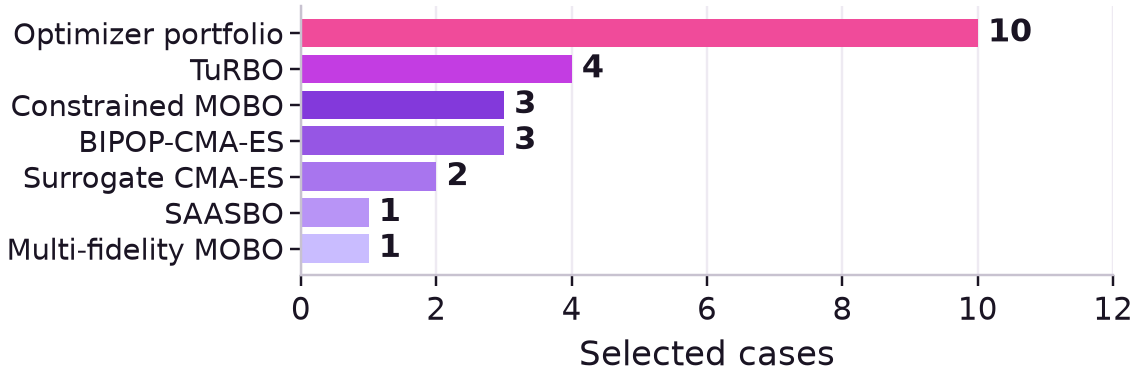
\includegraphics[width=6.50000in,height=2.16856in]{media/media/image6.png}

\emph{Figure 4. Archived tool distribution across the 24-case Evidence
2.4 and Prompt 1.1 development corpus; counts sum to the frozen 24-case
set and describe selection frequency rather than optimizer quality.}

\subsection{\texorpdfstring{\textbf{4.6 Synthetic integration
campaign}}{4.6 Synthetic integration campaign}}\label{synthetic-integration-campaign}

\emph{This verified proxy experiment is deliberately labeled
non-physical. It exercises compilation, candidate generation,
deterministic evaluation, persistence, selection, holdout accounting,
export, and evidence recomputation across ten scenario schemas. The local
adapter uses frozen seeds and coefficients; no PX4, Gazebo, vehicle
dynamics, network provider, or customer credential is involved. The
result tests orchestration and evidence flow only; it does not establish
controller quality, simulator fidelity, physical performance, deployment safety, or simulation-to-reality transfer.}

Simulation-queue behavior is also an experimental-validity concern.
Execution Claim Gate 1.1 binds each authorized Trial to a
content-addressed snapshot, while Scheduling Gate 1.0 admits the
least-served eligible Job's next FIFO Trial. Regressions cover
concurrent claimants, physical-attempt accounting, retry ownership, and
six alternating claims across two Jobs. These checks do not improve the
proxy objective; they prevent reported budgets and cohort comparisons
from being distorted by duplicate execution, starvation, or
shared-Runtime queue monopolization. The ledger retains every authorized
claim and terminal disposition for independent replay after every
failure, retry, and recovery.

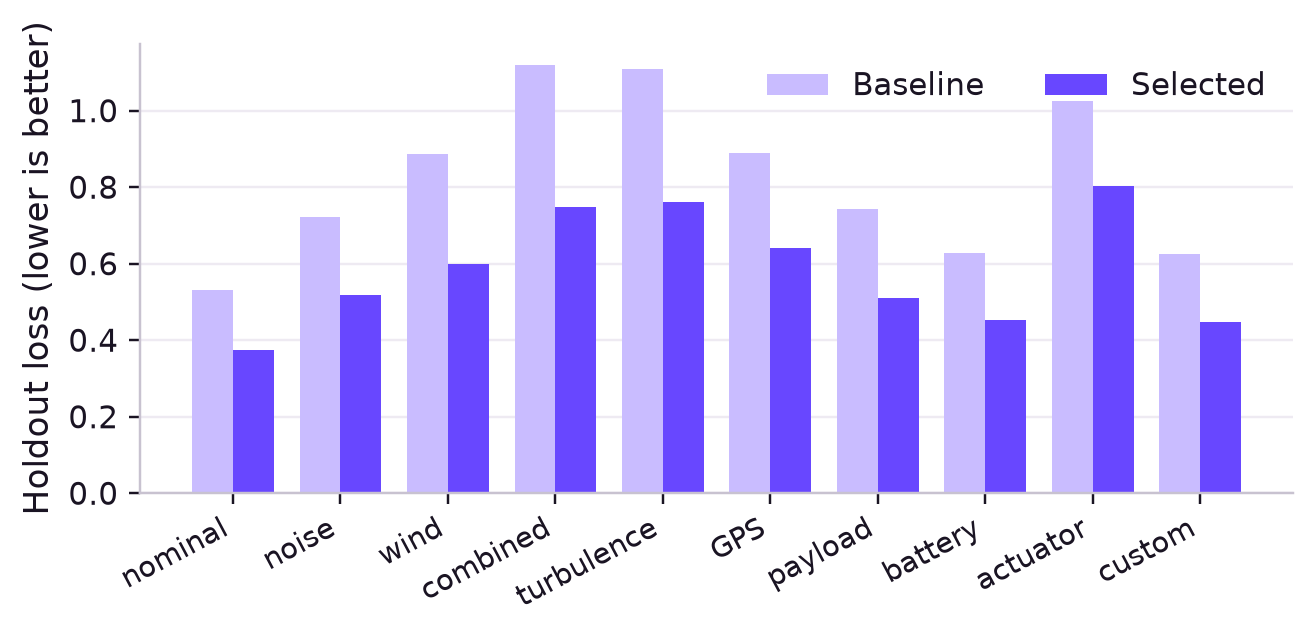
\includegraphics[width=5.00000in,height=2.41445in]{media/media/image7.png}

\emph{Figure 5. Baseline and selected holdout loss across ten frozen
synthetic scenarios; evidence metadata records a mock simulator, false
physical fidelity, and no provider network access.}

Across the frozen 61-candidate mock campaign, aggregate holdout loss
fell from 0.82811 to 0.58525 (29.327\% relative). All ten named
scenarios improved; scenario-wise relative reductions ranged from 21.8\%
to 33.2\%. The selected candidate matched the exhaustive mock oracle in
every scenario under the frozen proxy objective, candidate grid, and
deterministic tie-break rule. The exporter recomputes the aggregate and
per-scenario values from all persisted Trials and confirms that the
selected Candidate belongs to the evaluated set. These measurements
verify the closed synthetic campaign only; they do not predict the size
or direction of improvement in a physical simulator under any flight
condition.

The artifact declares physical\_fidelity=false, simulator\_backend=mock,
and provider\_network\_access=false. Its scenario scores are generated
by a frozen deterministic proxy objective rather than flight dynamics,
sensors, actuator models, or environmental plugins. The claim is limited
to orchestration, artifact completeness, and optimizer selection within
that proxy. It is not PX4/Gazebo evidence, real-aircraft evidence,
sim-to-real evidence, a safety claim, or a basis for physical deployment
decisions; any later physical claim
therefore requires independent, provenance-bound PX4/Gazebo
measurements under the frozen release protocol with matched seeds and
retained failures and independent recomputation externally.

\subsection{\texorpdfstring{\textbf{4.7 Scenario-wise proxy
behavior}}{4.7 Scenario-wise proxy behavior}}\label{scenario-wise-proxy-behavior}

Scenario-wise reporting exposes heterogeneity that a single aggregate
loss would conceal. The heat strip and the quantitative table use the
same ten frozen mock scenarios, selected Candidate, deterministic
objective, and persisted holdout records as the integration campaign
above. Values are paired within scenario: baseline and selected losses
are recomputed from the ledger before the relative reduction is
calculated. The resulting range shows that every declared proxy scenario
improved under this closed campaign, while preserving the same
non-physical boundary. These rows do not estimate uncertainty across
vehicles or simulators
and cannot be interpreted as PX4/Gazebo, real-aircraft, safety, or sim-to-real evidence.

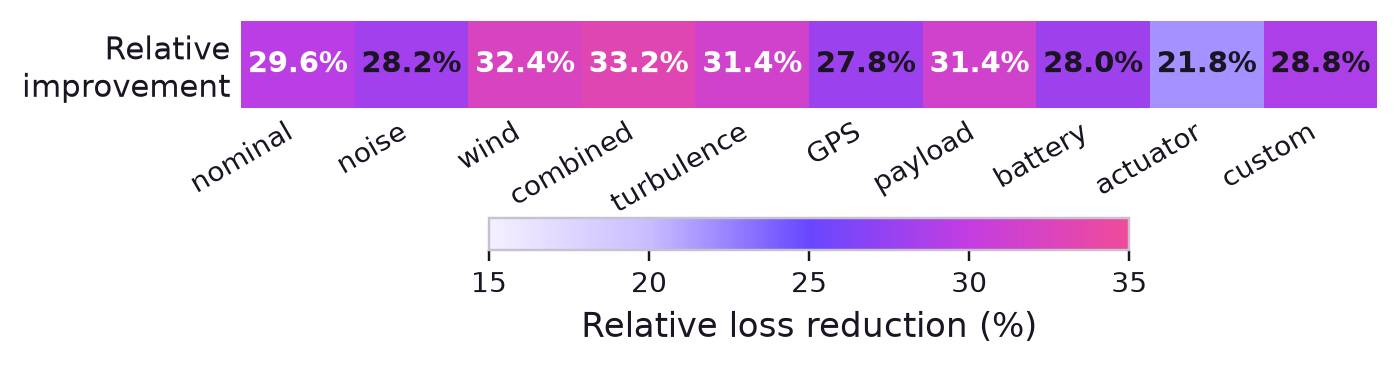
\includegraphics[width=6.50000in,height=1.25000in]{media/media/image8.png}

\emph{Figure 6. Relative loss reduction by mock scenario.}

The strip should be read as a paired descriptive view of the frozen
proxy campaign, not as a confidence interval or cross-vehicle
generalization result. Each cell recomputes the relative change from
the baseline and selected loss stored for the same named scenario, so a
row cannot borrow evidence from a different seed, scenario, or
Candidate. The narrow range is useful because it exposes whether one
scenario dominates the aggregate, yet it remains a property of this
deterministic mock objective. Publication-grade claims still require
independent seeds, physical simulator receipts, retained failures, and
uncertainty computed from the frozen PX4/Gazebo campaign rather than
synthetic proxy assumptions.

\begin{longtable}[]{@{}L{0.34\linewidth}C{0.18\linewidth}C{0.18\linewidth}C{0.18\linewidth}@{}}
\caption{Scenario-wise synthetic holdout results}\tabularnewline
\toprule
\textbf{Scenario} & \textbf{Baseline} & \textbf{Selected} &
\textbf{Reduction}\tabularnewline
\midrule
\endfirsthead
\toprule
\textbf{Scenario} & \textbf{Baseline} & \textbf{Selected} &
\textbf{Reduction}\tabularnewline
\midrule
\endhead
nominal & 0.5299 & 0.3733 & 29.55\%\tabularnewline
noise perturbed & 0.7221 & 0.5185 & 28.20\%\tabularnewline
wind perturbed & 0.8863 & 0.5992 & 32.39\%\tabularnewline
combined perturbed & 1.1193 & 0.7474 & 33.23\%\tabularnewline
turbulence & 1.1093 & 0.7609 & 31.41\%\tabularnewline
gps dropout & 0.8899 & 0.6422 & 27.83\%\tabularnewline
payload changed & 0.7429 & 0.5093 & 31.44\%\tabularnewline
battery degraded & 0.6288 & 0.4530 & 27.96\%\tabularnewline
actuator delay & 1.0262 & 0.8024 & 21.81\%\tabularnewline
custom & 0.6264 & 0.4463 & 28.75\%\tabularnewline
\bottomrule
\end{longtable}

\subsection{\texorpdfstring{\textbf{4.8 Physical scenario evidence
boundary}}{4.8 Physical scenario evidence boundary}}\label{physical-scenario-evidence-boundary}

Constant horizontal wind for the bundled x500 family has been verified
in a dedicated pinned WSL Runtime using PX4 commit
6ea3539157ca358c70a515878b77077af7d4611d and Gazebo 8.14.0. Acceptance
requires trial-local source hashes, exact /wind\_info read-back, and
expanded runtime SDF evidence for the spawned instance. The signed
installer Runtime has not yet passed this acceptance campaign, so the
capability is not yet a released-customer claim. Static-obstacle
injection has an implemented request and reply contract but awaits the
same signed-Runtime acceptance. Gust and turbulence, GPS or sensor
degradation, and battery, payload, or actuator-delay
effects remain outside every customer-Runtime or physical-performance
claim until complete simulator bindings, receipts, and acceptance evidence are frozen.
\looseness=-1

\begin{itemize}
\item
  Verified boundary --- constant horizontal wind for x500 is PX4\_GAZEBO
  evidence only inside the
  pinned dedicated WSL Runtime; the signed installer Runtime is still pending acceptance.
\item
  Implemented boundary --- static-obstacle injection and reply
  validation exist in source,
  but no released-customer performance claim is made before the signed-Runtime campaign passes.
\item
  Pending boundary --- gust, turbulence, GPS or sensor degradation,
  battery, payload, and actuator-delay effects remain excluded from
  physical claims until each has a complete binding, accepted receipt, and signed-Runtime evidence.
\end{itemize}

\section{\texorpdfstring{\textbf{5. Evaluation protocol for
publication-grade
results}}{5. Evaluation protocol for publication-grade results}}\label{evaluation-protocol-for-publication-grade-results}

The main benchmark will compare methods under the same pinned Runtime,
controller catalog, starting design, train/holdout split, trial budget,
failure thresholds, and blocked randomization schedule. Final-test
manifests must be frozen before any arm observes their outcomes. The
benchmark ledger must bind the Runtime image, simulator and controller
commits, scenario files, parameter domains, seed blocks, initial design,
stopping rule, failure-code mapping, and metric implementation. Each arm
receives equal access to training outcomes and identical terminal
accounting, while the final-test partition remains write-protected.
Reported aggregates must be independently recomputed from persisted
Trials with uncertainty, effect size, and failures retained in the
denominator. The same ledger must retain every excluded run and the
exact reason its result remained ineligible during external
recomputation and final publication stage.

The controlled comparison should progress from a default deterministic
policy to fixed CMA-ES, a specialist chosen before the final test, the
deterministic portfolio, an AURORA arm with recovery memory disabled,
and the complete AURORA system. Every arm must share the same scenario
set, initialization, trial budget, and terminal accounting. Specialist
selection must be frozen before final-test outcomes are visible,
portfolio comparisons require a matched exploration budget, and the
memory ablation must retain identical routing inputs. This sequence
isolates increasingly specific system contributions without treating a
method-name difference as causal evidence or attributing it to AURORA
without evidence.

\begin{itemize}
\item
  Primary outcomes: frozen holdout
  loss, feasible-campaign rate, baseline improvement, time-to-target,
  and terminal failure rate with uncertainty for every reported arm and
  seed block.
\item
  Secondary outcomes: wall time, model tokens and cost, router latency,
  recovery success, scenario-wise regret, and artifact completeness for
  every frozen comparison arm and seed block.
\item
  Use at least five independent seeds for engineering diagnostics and
  preferably ten for
  report-level comparisons across every reported arm before any superiority claim is published.
\item
  Keep failures in the denominator; do not impute a successful loss.
\item
  Report uncertainty
  and effect sizes; never publish superiority from one seed or one track.
\end{itemize}

\section{\texorpdfstring{\textbf{6. Product reliability and
operations}}{6. Product reliability and operations}}\label{product-reliability-and-operations}

The desktop readiness gate is part of the product's technical contract.
The progress bar may reach 100\% only after every check that DroneDream
can perform at launch has reached a terminal pass state. The entry
action must not become visible while a required check is pending or
failed. After entry, runtime failures still need explicit diagnostics
because network loss, disk damage, permission changes, and external
service changes cannot be permanently prevented. The gate therefore
certifies a timestamped launch snapshot rather than promising an
error-free future session, and post-entry faults must remain recoverable,
attributable, and visible without silently invalidating prior work for
every affected run.

\textbf{Readiness is a conjunction, not a progress animation.} The
launcher requires a fresh supported-system probe, one owned and
compatible Runtime, a healthy local service, no mandatory update, and an
account accepted by the local API. Missing, stale, mismatched,
unreachable, or still-checking states remain blocking. Only the current
gate may set the bar to 100\%, change the environment badge to CHECKED,
and reveal the entry action. Quantitative release evidence still needs
time-to-ready
p50/p95, false-ready rate, and a clean Windows/upgrade matrix across
fresh install, upgrade, repair, and duplicate-download paths before any
release is accepted for public distribution on a supported Windows
architecture.

\textbf{Exit and account operations use the same recoverability
principle.} Closing warns about an active simulation or unsaved draft,
stops work that cannot survive process termination, and preserves a
recoverable draft whenever possible without trapping the user in the
application. Managed-model usage consumes the included quota through a
server-side ledger before BYOK is required; provider receipts must later
be reconciled against that ledger. Remaining evidence therefore concerns
draft-recovery and exit success rates plus quota-receipt consistency,
not a new product capability claim, across every managed-provider
transaction, recovery path, and audit replay retained by the service
ledger.

\section{\texorpdfstring{\textbf{7. Limitations and next
experiments}}{7. Limitations and next experiments}}\label{limitations-and-next-experiments}

AURORA's present evidence establishes enforceable software boundaries
and reproducible mock-campaign behavior, but it does not yet establish
broad optimization superiority or customer-Runtime physical-simulator
performance. The distinctions below are active claim constraints, not
generic future-work disclaimers: each one identifies the evidence unit
that is missing, the confounder that remains uncontrolled, or the
environment that has not been accepted. Keeping those boundaries
explicit prevents development routing accuracy, deterministic guard
probes, and synthetic proxy gains from being combined into a stronger
conclusion than their protocols support. The next experiments are
therefore ordered around frozen matched budgets, independent
recomputation, signed Runtime acceptance, and scenario-level uncertainty
over time.

\begin{itemize}
\item
  No
  result in this report establishes real-aircraft safety, certification, or direct sim-to-real transfer.
\item
  The archived 24-case online routing corpus qualifies Evidence 2.4 and
  Prompt 1.1 only; Evidence 2.7 and
  Prompt 1.5 require a fresh online provider freeze before current
  routing qualification against the revised prompt schema.
\item
  The current 16-case policy holdout verifies deterministic eligibility
  only; its published labels are not permanently blind and require a
  future concealed benchmark with sealed labels.
\item
  The source-contract ablation demonstrates named guard behavior, not
  causal optimization-quality lift.
\item
  The frozen four-arm mock ablation changes protocol-level behavior in
  15/15 full-arm comparisons, but its 5/5 receipt-only-memory isolations
  remain inconclusive under the scripted policy and do not authorize a
  general causal or optimizer-superiority claim across broader
  optimizer families or deployment conditions.
\item
  The 10/10 fallback result verifies deterministic recovery on a
  frozen mock protocol, not that AURORA improves objective value beyond
  recovery equivalence or supports causal attribution.
\item
  The ten-scenario campaign is synthetic mock evidence, not physical
  scenario coverage.
\item
  The
  pinned steady-wind result is not yet accepted in the signed customer Runtime.
\item
  Publication-grade optimizer comparisons, physical component
  ablations, multi-seed confidence intervals, cost/latency measurements,
  and UX telemetry remain pending before customer qualification.
\item
  External baselines such as expert manual tuning or PX4 AutoTune must
  be included only when controller, vehicle, track, budget, metrics, and
  failure accounting are genuinely aligned.
\end{itemize}

\subsection{\texorpdfstring{\textbf{7.1 Threats to
validity}}{7.1 Threats to validity}}\label{threats-to-validity}

The report's evidence units answer different questions and cannot be
pooled into one score. Routing cases measure tool eligibility; source
probes test whether named guards reject constructed violations; fallback
arms measure recovery equivalence; and synthetic scenarios measure a
deterministic proxy. Substituting one unit for another creates a
construct-validity error even when all recorded values are correct.
Because the same implementation sometimes generates, executes, and
verifies an artifact, the next campaign also requires independent
recomputation, immutable manifests, negative controls, and failure
injection before an optimization-quality comparison is described as
causal in publication.

Statistical validity requires the scenario, not an optimizer Trial, to
remain the primary comparison unit. Trials in one trajectory share
initialization, history, stopping conditions, and candidate ancestry, so
treating them as independent understates uncertainty. A publication
result must freeze seed blocks, report paired scenario-wise differences,
retain terminal failures in the denominator, and present effect sizes
with intervals rather than one aggregate percentage. Hyperparameters,
method choice, and stopping rules must be fixed before the final
partition opens;
exploratory findings remain useful but cannot replace the frozen
confirmatory comparison across every arm or its reported causal
estimate.

Operational reproducibility requires more than code and a controller
vector. A repeatable run must bind the owned Runtime image, PX4/Gazebo
commits, vehicle and world assets, controller schema, scenario manifest,
optimizer settings, seeds, environment, and evidence verifier. It must
retain cancellations, timeouts, rejected callbacks, and post-launch
changes rather than successful Trials alone. The ledger already supplies
the source commit, test totals, digests, and reproduction command; the
remaining gap is a signed customer-Runtime
campaign executable on another machine without repository-specific
state, hidden assumptions, operator interpretation, or independent
auditability during replay.

External validity is bounded by controller, vehicle, world, and
disturbance combinations actually executed. Many Trials in one x500
setup do not cover fixed-wing vehicles, payload changes, actuator
saturation, estimator faults, or other controller structures. A broader
benchmark therefore needs a declared scenario matrix with held-out
combinations, not a convenient collection of worlds. Every cell must
explain its distinct operating condition, mutable parameters, and
invariant feasibility constraints. Results must be aggregated within and
across vehicle families so a strong
mean cannot conceal a systematic failure in one operationally important
subgroup or declared scenario family under final evaluation.

Measurement validity also requires more than scalar holdout loss. The
protocol must retain trajectory error, settling time, overshoot, control
effort, saturation, constraint violations, termination cause, and
wall-clock cost, with units, sampling rules, preprocessing versions, and
direction of improvement. A controller can lower an aggregate score by
accepting oscillation or excessive actuator demand, so feasibility
remains a gate rather than a narrative caveat. Primary metrics and
admissibility rules must be registered before optimization, while
diagnostics remain visible for failure
analysis; post-hoc metric choice cannot redefine a failed campaign as
successful after execution once final outcomes become visible.

The next campaign prioritizes fixed-budget PX4/Gazebo outcomes,
physical component-level AURORA ablations, failure injection, and the
readiness/exit matrix. It freezes the Runtime, controller catalog,
scenario manifests, seed blocks, budgets, eligibility policy, and
terminal taxonomy before any final arm runs. Matched baselines include
fixed CMA-ES, a preselected specialist, the deterministic portfolio, and
isolated AURORA variants. Signed JSON and CSV artifacts will replace
planned result sections without
hiding failures or inflating evidence beyond its physical and
statistical boundaries. The retained ledger must also show which
planned comparisons never executed and why in the retained receipt.

\section{\texorpdfstring{\textbf{8. Reproducibility and source
ledger}}{8. Reproducibility and source ledger}}\label{reproducibility-and-source-ledger}

Figures 2--6 trace to evidence bundle v6, canonical SHA-256 prefix
\texttt{bd99720f50a63d28}; Figure 1 is a schematic. The bundle binds
software subject \texttt{0429b42}, provenance \texttt{738157c}, and
head \texttt{a0040d4}. Its backend receipt records 1,139/1,139 tests in
759.17 seconds on a pre-commit worktree, not an exact-final run; 59
affected checks passed on the subject. Ruff and mypy are unreceipted,
and Windows Rust was not run. The website receipt links
\texttt{a64f995} to \texttt{943f3b6} and records 322/322 tests,
typecheck, lint, build, nine deployment tests, and deterministic
117-file output across two builds. The reference manifest verifies both
chains without copying raw evidence; its companion receipt binds report
source, PDF, audits, and the reproduction command needed for
deterministic regeneration and independent review after release.

Execution Claim Gate 1.1 and Outcome Contract 2.20 bind the
Trial/Candidate/Job snapshot and
authorized scenario matrix; drift fails closed before evidence
admission. Concurrent claims retain one accepted physical attempt, and
least-served per-Job scheduling prevents large-experiment queue
monopolization. Prompt Schema 2.3 gives same-type training cases
separate provider-safe aliases while sealing raw case IDs and holdout
evidence. Evidence 2.7 and Prompt 1.5 add verified observational outcome
reflection, while the archived online artifact passed 24/24 only under
Evidence 2.4 and Prompt 1.1. The current deterministic eligibility
artifact passed 16/16 policy-holdout cases without network or model
calls; a fresh online provider freeze is still required for the revised
contract. The fallback campaign persisted 579 Trials across 15 Jobs and
matched the direct arm in 10/10 frozen block comparisons. The
accompanying machine-readable audit retains source hashes, reproduction
commands, qualification scope, and per-artifact provenance required for
independent regeneration from the frozen release artifact and its
independently verified claim boundary for replay and release review
{[}\protect\hyperlink{ref_1}{\emph{1}}{]}.

\section{\texorpdfstring{\textbf{9.
Conclusion}}{9. Conclusion}}\label{conclusion}

DroneDream 1.0 positions AURORA as an evidence-gated Harness for UAV
controller optimization in simulation: model reasoning interprets intent
and coordinates eligible methods, while deterministic contracts retain
authority over inputs, execution, evidence admission, and completion.
The frozen release demonstrates the exercised software boundaries
through routing, holdout-policy, guard-ablation, fallback-equivalence,
claim-receipt, and case-separated feedback checks; it does not convert
those checks into a claim of real-aircraft safety or general simulator
superiority. The next decisive step is a signed customer-Runtime
PX4/Gazebo campaign with frozen scenario manifests, matched budgets,
paired seeds, retained failures, and independent recomputation. That
campaign can test optimization quality and operational reproducibility
without weakening the provenance and leakage boundaries already enforced
by AURORA in later studies.

The current release therefore changes what future experiments can safely
assert before it changes the empirical flight result itself. Claim v3,
Outcome Contract 2.20, input/outcome/scenario drift rejection, and
cross-Job fair scheduling make concurrent attempt counts, parameter
provenance, and scenario eligibility independently auditable. A decisive
external campaign must still freeze PX4/Gazebo versions, manifests, seed
blocks, budgets, metrics, and baseline arms before execution; retain
every timeout and failed Trial; and recompute signed outcomes outside
the application process. This separation keeps AURORA's demonstrated
software assurances distinct from the optimization-quality claims that
only the
next physical simulator study can establish under the frozen evaluation
protocol without ambiguity.

\section{\texorpdfstring{\textbf{References}}{References}}\label{references}

References follow IEEE numeric order, and every body citation links to
its entry. External sources establish method lineage and evaluation
conventions; no external benchmark value is imported into DroneDream
evidence. Online sources include a July 2026 access date. A citation
establishes lineage, not implementation; the frozen source ledger
remains authoritative for every DroneDream capability and reported
measurement. Implementation claims therefore require corresponding
source paths,
executable tests, and release evidence under the same frozen commit.

\begin{multicols}{2}
\footnotesize
\setlength{\parskip}{0.08em}
\setlength{\columnsep}{1.15em}

\protect\hypertarget{ref_1}{}{}{[}1{]} DroneDream, ``Release evidence
ledger,'' ver. 1.0, evidence bundle v6, software subject
\texttt{0429b42}, Jul. 2026.

\protect\hypertarget{ref_2}{}{}{[}2{]} PX4 Development Team,
``Multicopter PID tuning guide (manual/basic),'' PX4 User Guide, 2026.
{[}Online{]}. {[}Accessed: Jul. 27, 2026{]}. Available:
\href{https://docs.px4.io/main/en/config_mc/pid_tuning_guide_multicopter_basic}{\emph{PX4
Docs}}

\protect\hypertarget{ref_3}{}{}{[}3{]} PX4 Development Team,
``Simulation,'' PX4 User Guide, 2026. {[}Online{]}. {[}Accessed: Jul.
27, 2026{]}. Available:
\href{https://docs.px4.io/main/en/simulation/}{\emph{PX4 Docs}}

\protect\hypertarget{ref_4}{}{}{[}4{]} N. Hansen and A. Ostermeier,
``Completely derandomized self-adaptation in evolution strategies,''
Evol. Comput., vol. 9, no. 2, pp. 159--195, 2001, doi:
10.1162/106365601750190398.
\href{https://doi.org/10.1162/106365601750190398}{\emph{DOI}}

\protect\hypertarget{ref_5}{}{}{[}5{]} D. Golovin et al., ``Google
Vizier: A service for black-box optimization,'' in Proc. 23rd ACM SIGKDD
Int. Conf. Knowl. Discovery Data Mining, 2017, pp. 1487--1495, doi:
10.1145/3097983.3098043.
\href{https://doi.org/10.1145/3097983.3098043}{\emph{DOI}}

\protect\hypertarget{ref_6}{}{}{[}6{]} M. Balandat et al., ``BoTorch: A
framework for efficient Monte-Carlo Bayesian optimization,'' in Adv.
Neural Inf. Process. Syst., vol. 33, pp. 21524--21538, 2020.
\href{https://arxiv.org/abs/1910.06403}{\emph{arXiv}}

\protect\hypertarget{ref_7}{}{}{[}7{]} D. Eriksson et al., ``Scalable
global optimization via local Bayesian optimization,'' in Adv. Neural
Inf. Process. Syst., vol. 32, 2019.
\href{https://arxiv.org/abs/1910.01739}{\emph{arXiv}}

\protect\hypertarget{ref_8}{}{}{[}8{]} D. Eriksson and M. Jankowiak,
``High-dimensional Bayesian optimization with sparse axis-aligned
subspaces,'' in Proc. 37th Conf. Uncertainty Artif. Intell., 2021, pp.
493--503. \href{https://arxiv.org/abs/2103.00349}{\emph{arXiv}}

\protect\hypertarget{ref_9}{}{}{[}9{]} A. Brohan et al., ``RT-1:
Robotics Transformer for real-world control at scale,''
arXiv:2212.06817, 2022.
\href{https://arxiv.org/abs/2212.06817}{\emph{arXiv}}

\protect\hypertarget{ref_10}{}{}{[}10{]} A. Brohan et al., ``RT-2:
Vision-language-action models transfer Web knowledge to robotic
control,'' in Proc. 7th Conf. Robot Learning, 2023.
\href{https://arxiv.org/abs/2307.15818}{\emph{arXiv}}

\protect\hypertarget{ref_11}{}{}{[}11{]} Open X-Embodiment Collaboration
et al., ``Open X-Embodiment: Robotic learning datasets and RT-X
models,'' in Proc. IEEE Int. Conf. Robot. Autom., 2024.
\href{https://arxiv.org/abs/2310.08864}{\emph{arXiv}}

\protect\hypertarget{ref_12}{}{}{[}12{]} M. J. Kim et al., ``OpenVLA: An
open-source vision-language-action model,'' arXiv:2406.09246, 2024.
\href{https://arxiv.org/abs/2406.09246}{\emph{arXiv}}

\protect\hypertarget{ref_13}{}{}{[}13{]} K. Black et al., ``π0: A
vision-language-action flow model for general robot control,''
arXiv:2410.24164, 2024.
\href{https://arxiv.org/abs/2410.24164}{\emph{arXiv}}

\protect\hypertarget{ref_14}{}{}{[}14{]} Physical Intelligence et al.,
``π0.5: A vision-language-action model with open-world generalization,''
arXiv:2504.16054, 2025.
\href{https://arxiv.org/abs/2504.16054}{\emph{arXiv}}

\protect\hypertarget{ref_15}{}{}{[}15{]} C. Zhang et al., ``JoyAI-RA
0.1: A foundation model for robotic autonomy,'' arXiv:2604.20100, 2026.
\href{https://arxiv.org/abs/2604.20100}{\emph{arXiv}}

\protect\hypertarget{ref_16}{}{}{[}16{]} J. Yang et al., ``SWE-agent:
Agent-computer interfaces enable automated software engineering,'' in
Adv. Neural Inf. Process. Syst., vol. 37, 2024.
\href{https://arxiv.org/abs/2405.15793}{\emph{arXiv}}

\protect\hypertarget{ref_17}{}{}{[}17{]} A. Novikov et al.,
``AlphaEvolve: A Gemini-powered coding agent for designing advanced
algorithms,'' arXiv:2506.13131, 2025.
\href{https://arxiv.org/abs/2506.13131}{\emph{arXiv}}

\protect\hypertarget{ref_18}{}{}{[}18{]} DeepSeek-AI, ``DeepSeek-V3
technical report,'' arXiv:2412.19437, 2024.
\href{https://arxiv.org/abs/2412.19437}{\emph{arXiv}}

\protect\hypertarget{ref_19}{}{}{[}19{]} A. Yang et al., ``Qwen2
technical report,'' arXiv:2407.10671, 2024.
\href{https://arxiv.org/abs/2407.10671}{\emph{arXiv}}

\protect\hypertarget{ref_20}{}{}{[}20{]} K. Bousmalis et al., ``RoboCat:
A self-improving generalist agent for robotic manipulation,'' Trans.
Mach. Learn. Res., 2023.
\href{https://arxiv.org/abs/2306.11706}{\emph{arXiv}}

\protect\hypertarget{ref_21}{}{}{[}21{]} O. M. Team et al., ``Octo: An
open-source generalist robot policy,'' in Proc. Robotics: Science and
Systems, 2024. \href{https://arxiv.org/abs/2405.12213}{\emph{arXiv}}

\protect\hypertarget{ref_22}{}{}{[}22{]} H. Walke et al., ``BridgeData
V2: A dataset for robot learning at scale,'' in Proc. Conf. Robot
Learning, 2023. \href{https://arxiv.org/abs/2308.12952}{\emph{arXiv}}

\protect\hypertarget{ref_23}{}{}{[}23{]} A. Khazatsky et al., ``DROID: A
large-scale in-the-wild robot manipulation dataset,'' in Proc. Robotics:
Science and Systems, 2024.
\href{https://arxiv.org/abs/2403.12945}{\emph{arXiv}}

\protect\hypertarget{ref_24}{}{}{[}24{]} A. Nasiriany et al.,
``RoboCasa: Large-scale simulation of everyday tasks for generalist
robots,'' in Proc. Robotics: Science and Systems, 2024.
\href{https://arxiv.org/abs/2406.02523}{\emph{arXiv}}

\protect\hypertarget{ref_25}{}{}{[}25{]} Y. Chen et al., ``RoboTwin 2.0:
A scalable data generator and benchmark with strong domain randomization
for robust bimanual robotic manipulation,'' arXiv:2506.18088, 2025.
\href{https://arxiv.org/abs/2506.18088}{\emph{arXiv}}

\protect\hypertarget{ref_26}{}{}{[}26{]} AgiBot-World Contributors et
al., ``AgiBot World Colosseo: A large-scale manipulation platform for
scalable and intelligent embodied systems,'' arXiv:2503.06669, 2025.
\href{https://arxiv.org/abs/2503.06669}{\emph{arXiv}}

\protect\hypertarget{ref_27}{}{}{[}27{]} C. Chi et al., ``Diffusion
Policy: Visuomotor policy learning via action diffusion,'' Int. J.
Robot. Res., vol. 42, no. 13, pp. 1172--1198, 2023.
\href{https://arxiv.org/abs/2303.04137}{\emph{arXiv}}

\protect\hypertarget{ref_28}{}{}{[}28{]} S. Yao et al., ``ReAct:
Synergizing reasoning and acting in language models,'' in Proc. Int.
Conf. Learn. Representations, 2023.
\href{https://arxiv.org/abs/2210.03629}{\emph{arXiv}}

\protect\hypertarget{ref_29}{}{}{[}29{]} T. Schick et al., ``Toolformer:
Language models can teach themselves to use tools,'' in Adv. Neural Inf.
Process. Syst., vol. 36, 2023.
\href{https://arxiv.org/abs/2302.04761}{\emph{arXiv}}

\protect\hypertarget{ref_30}{}{}{[}30{]} N. Shinn et al., ``Reflexion:
Language agents with verbal reinforcement learning,'' in Adv. Neural
Inf. Process. Syst., vol. 36, 2023.
\href{https://arxiv.org/abs/2303.11366}{\emph{arXiv}}

\protect\hypertarget{ref_31}{}{}{[}31{]} D. R. Jones, M. Schonlau, and
W. J. Welch, ``Efficient global optimization of expensive black-box
functions,'' J. Global Optim., vol. 13, no. 4, pp. 455--492, 1998, doi:
10.1023/A:1008306431147.
\href{https://doi.org/10.1023/A:1008306431147}{\emph{DOI}}

\protect\hypertarget{ref_32}{}{}{[}32{]} J. Snoek, H. Larochelle, and R.
P. Adams, ``Practical Bayesian optimization of machine learning
algorithms,'' in Adv. Neural Inf. Process. Syst., vol. 25, 2012.
\href{https://arxiv.org/abs/1206.2944}{\emph{arXiv}}

\protect\hypertarget{ref_33}{}{}{[}33{]} B. Shahriari, K. Swersky, Z.
Wang, R. P. Adams, and N. de Freitas, ``Taking the human out of the
loop: A review of Bayesian optimization,'' Proc. IEEE, vol. 104, no. 1,
pp. 148--175, Jan. 2016, doi: 10.1109/JPROC.2015.2494218.
\href{https://arxiv.org/abs/1502.05700}{\emph{arXiv}}

\end{multicols}
\normalsize

\section{\texorpdfstring{\textbf{Appendix A. Release-contract
verification}}{Appendix A. Release-contract verification}}\label{appendix-a.-release-contract-verification}
\setlength{\LTpre}{0.35em}
\setlength{\LTpost}{0.35em}

The verification matrix separates executable software evidence from
broader product claims. It covers protected state mutations,
authenticated report export and watermark behavior, frontend command
wiring, rendered layout, and Python static checks. Every count describes
the checked release contract at this source boundary; none measures
controller quality, physical simulator fidelity, real-flight safety, or
causal optimization benefit. The matrix also gives reviewers a compact
map from each reported count to the narrow claim it can support.
It therefore separates release verification from every physical or
optimizer-performance conclusion and related claim in the report.
Unsupported cells remain unavailable instead of being normalized into a
passing result or presented as verified engineering evidence at this
release boundary.

\begin{longtable}[]{@{}L{0.28\linewidth}C{0.12\linewidth}C{0.12\linewidth}L{0.38\linewidth}@{}}
\caption{Release-contract verification matrix}\tabularnewline
\toprule
\textbf{Verification surface} & \textbf{Cases} & \textbf{Passed} &
\textbf{Claim boundary}\tabularnewline
\midrule
\endfirsthead
\toprule
\textbf{Verification surface} & \textbf{Cases} & \textbf{Passed} &
\textbf{Claim boundary}\tabularnewline
\midrule
\endhead
State-version fence & 5 & 5 & Protected Job/Batch
mutations\tabularnewline
Report export contract & 51 & 51 & Tier, watermark, iteration
trace\tabularnewline
Frontend validation receipt & 322 & 322 & Tests plus
typecheck/lint/build\tabularnewline
Report layout contract & Recomputed & Required & Rendered body/list
policy\tabularnewline
Backend validation receipt & 1,139 & 1,139 & Pre-commit full run;
59-check subject bridge\tabularnewline
\bottomrule
\end{longtable}

\subsection{\texorpdfstring{\textbf{A.1 Experiment-report and reflection
evidence
policy}}{A.1 Experiment-report and reflection evidence policy}}\label{a.1-experiment-report-and-reflection-evidence-policy}

A downloadable tuning report is a projection of retained experiment
evidence, not a newly inferred narrative. It retains generation
ancestry, parameter deltas, metrics, terminal Trial counts, and proposal
rationale; missing lineage remains unavailable instead of being
reconstructed from a favorable outcome. The authenticated server
snapshot resolves export tier and prevents redirect-based entitlement
bypass. Reflection follows the same fail-closed rule: an execution
receipt must match the exact modern Candidate cohort before AURORA
exposes completion, accepted work, domain failures, feasibility,
incumbent change, or observed improvement. Any legacy, incomplete, or
drifted cohort makes the block unavailable; holdout values stay sealed,
zero-dispatch decisions remain not applicable, and observations never
become causal tool credit.

\subsection{\texorpdfstring{\textbf{A.2 Frozen report
projection}}{A.2 Frozen report projection}}\label{a.2-frozen-report-projection}

The report exporter reconstructs an experiment from persisted evidence
rather than from the current user interface state. Its input boundary
contains the Job specification, ordered Candidate generations,
parameter snapshots, objective and constraint metrics, terminal Trial
taxonomy, proposal rationale, and the exact export entitlement resolved
by the authenticated server. It records attempted iterations, admitted
observations, parameter changes, and the Candidate frozen for holdout
review. Missing receipts remain unavailable, failed Trials stay in the
denominator, and no prose generator may invent a cause absent from the
retained ledger. The result is a portable audit view of the completed
campaign, including its failed and unavailable observations, rather than a detached narrative of success.
\looseness=-1

For Free accounts, the renderer places one native vector seal on every
page after pagination is final. The seal is drawn with the DroneDream
violet-magenta identity at eighteen percent opacity, intersects the body
without covering it, and remains present after ordinary PDF extraction
or printing. Plus and Pro exports omit the mark only when the server-side
entitlement snapshot authorizes unwatermarked bytes. Redirect URLs,
stale desktop state, or a modified client request cannot change that
decision. Fifty-one contract cases cover tier resolution, watermark
cardinality, iteration trace, missing-evidence behavior, and stable byte
generation. Their authority ends at export correctness; they do not
qualify controller quality, simulator performance, or real-aircraft
behavior under any simulated or physical evaluation.

\subsection{\texorpdfstring{\textbf{A.3 Qualification
handoff}}{A.3 Qualification handoff}}\label{a.3-qualification-handoff}

A report-level claim advances only when its evidence class, prompt
schema, source commit, Runtime identity, and acceptance command are
frozen together. Evidence 2.7 and Prompt 1.5 therefore require a fresh
provider campaign and cannot inherit the archived 24/24 routing score.
Physical qualification must likewise use matched budgets and paired
seeds in the signed Runtime, retain failures, bind PX4/Gazebo commits,
and independently recompute persisted outcomes. Until those gates pass,
AURORA's verified claim remains narrow: software contracts constrain
experiment formation, routing, execution, reflection, recovery, export,
and freeze; they do not establish optimizer superiority, physical-simulator fidelity, or flight performance.
\looseness=-1

\subsection{\texorpdfstring{\textbf{A.4 Frozen component outcome
ablation}}{A.4 Frozen component outcome ablation}}\label{a.4-frozen-component-outcome-ablation}

The preregistered offline ablation locks five seed blocks across full
AURORA, no decision memory, no observed-outcome reflection, and a fixed
portfolio. Its 20 Jobs persist 554 Trials with complete evidence, zero
network calls, and no real credential. Across the 15 paired arm
comparisons, five expose an observed protocol difference and ten show no
observed protocol difference under the frozen local router. The five
receipt-only-memory isolations remain explicitly inconclusive rather
than being converted into a causal component claim under this
deliberately bounded offline decision protocol.
\looseness=-1

\begingroup
\footnotesize
\renewcommand{\arraystretch}{1.22}
\setlength{\LTpre}{0.60em}
\begin{longtable}[]{@{}L{0.25\linewidth}C{0.08\linewidth}C{0.10\linewidth}L{0.30\linewidth}L{0.13\linewidth}@{}}
\caption{Frozen four-arm component outcome ablation}\tabularnewline
\toprule
\textbf{Arm} & \textbf{Jobs} & \textbf{Trials} &
\textbf{Tool sequence} & \textbf{Finding}\tabularnewline
\midrule
\endfirsthead
\toprule
\textbf{Arm} & \textbf{Jobs} & \textbf{Trials} &
\textbf{Tool sequence} & \textbf{Finding}\tabularnewline
\midrule
\endhead
Full AURORA & 5 & 120 & constrained MOBO to TuRBO & Reference\tabularnewline
No decision memory & 5 & 120 & constrained MOBO to portfolio & No observed difference\tabularnewline
No outcome reflection & 5 & 120 & constrained MOBO to portfolio & No observed difference\tabularnewline
Fixed portfolio & 5 & 194 & portfolio to portfolio & Observed difference\tabularnewline
Receipt-only isolation & 5 pairs & --- & matched route and outcome & Inconclusive\tabularnewline
\bottomrule
\end{longtable}
\endgroup

\subsection{\texorpdfstring{\textbf{A.5 Phase-qualified execution
surface}}{A.5 Phase-qualified execution surface}}\label{a.5-phase-qualified-execution-surface}

Capability eligibility answers whether a tool can honor the declared Job
shape; the phase policy independently answers whether that tool should
be executable now. Evidence 2.7 intersects the capability-qualified set
with the receding-plan phase before schema generation, provider
manifest construction, response validation, trace verification, or
dispatch. Prompt 1.5 and Decision Trace 1.3 therefore persist the exact
surface shown to the model. Every phase retains the deterministic
portfolio fallback, and a response naming any filtered tool is rejected
rather than repaired into an executable decision. The retained trace
therefore explains every admitted and excluded tool during later replay
and independent review.

Fidelity remains a separate execution contract. Multi-fidelity methods
may screen Candidates below full fidelity during exploration or
diversification, but a verification decision forces every
reduced-fidelity-capable strategy to fidelity 1.0. The final generation
and last available capacity also preserve a full-fidelity path, while
the ordinary acceptance, claim-receipt, scenario, and holdout gates
remain unchanged. This prevents an inexpensive screening outcome from
becoming the final winner merely because its optimizer was otherwise
eligible for the current Job and scenario profile. The receipt must
therefore record both screening fidelity and the full-fidelity
verification used for terminal selection.

\begin{longtable}[]{@{}L{0.21\linewidth}C{0.13\linewidth}L{0.34\linewidth}L{0.22\linewidth}@{}}
\caption{Phase-qualified search-role surface}\tabularnewline
\toprule
\textbf{Plan phase} & \textbf{Role count} & \textbf{Primary search intent} &
\textbf{Fidelity rule}\tabularnewline
\midrule
\endhead
Exploration & 6 & Global, sparse, and multi-fidelity discovery &
Budget policy\tabularnewline
Recovery & 4 & Restart and deterministic recovery &
Budget policy\tabularnewline
Refinement & 5 & Local and surrogate exploitation &
Budget policy\tabularnewline
Diversification & 7 & Broad escape from stalled regions &
Budget policy\tabularnewline
Verification & 5 & Confirm the strongest eligible Candidate &
\textbf{Fidelity 1.0}\tabularnewline
Balanced & 8 & Preserve the complete qualified registry &
Budget policy\tabularnewline
\bottomrule
\end{longtable}

\subsection{\texorpdfstring{\textbf{A.6 Evidence-source
ledger}}{A.6 Evidence-source ledger}}\label{a.6-evidence-source-ledger}

Every quantitative statement routes through one named artifact rather
than console output or reconstructed prose. The exporter verifies each
file, recomputes its aggregate, and records the evidence class. Router
rows therefore support eligibility claims only; mock campaigns support
bounded software and synthetic-response claims; component ablations
support observed protocol differences under their frozen offline
router. Backend and frontend receipts establish software validation,
not provider, PX4/Gazebo, or real-flight qualification. A reviewer can
therefore reproduce each number while seeing which stronger conclusion
remains unauthorized under the declared evidence boundary and receipt.

\begingroup
\footnotesize
\renewcommand{\arraystretch}{1.06}
\setlength{\LTpre}{0.30em}
\setlength{\LTpost}{0.20em}
\begin{longtable}[]{@{}L{0.25\linewidth}C{0.15\linewidth}L{0.22\linewidth}L{0.28\linewidth}@{}}
\caption{Evidence-source and claim-boundary ledger}\tabularnewline
\toprule
\textbf{Evidence surface} & \textbf{Scale} &
\textbf{Source ID} & \textbf{Authorized claim}\tabularnewline
\midrule
\endhead
Policy holdout & 16/16 & Policy holdout v3 &
Eligibility-set determinism\tabularnewline
Source-contract ablation & 25/25 vs.\ 6/25 & Contract ablation v1 &
Fail-closed guard behavior\tabularnewline
Fallback outcome campaign & 15 Jobs, 579 Trials & Fallback campaign v1 &
Matched offline recovery\tabularnewline
Component outcome ablation & 20 Jobs, 554 Trials & Component ablation v1 &
Observed protocol differences\tabularnewline
Synthetic scenario campaigns & 2 $\times$ 61 Candidates &
Coverage v3 / generalization v1 &
Seed and mixed-shift reporting\tabularnewline
\bottomrule
\end{longtable}
\endgroup
